
%=====================================================================
\section{Prime-fire reduction and periodic selector regimes}\label{sec:fire}
%=====================================================================
\subsection{Prime-fire reduction}
A prime-fire step at $x$ chooses a prime $p\mid x$ and moves to $T_p(x)=x(p+1)^2/p$. By Theorem~\ref{thm:valuation} it lowers $v_p$ by one and raises $v_q$ by $2v_q(p+1)$ for the primes $q\mid p+1$. The following fact about those primes is the whole mechanism.
\begin{lemma}[Primes of $p+1$]\label{lem:pplus1}
If $p\ge5$ is prime and $q$ is a prime dividing $p+1$, then $q<p$. For $p=2$ the only such prime is $3$, and for $p=3$ it is $2$.
\end{lemma}
\begin{proof} For $p\ge5$ the number $p+1$ is even and $q\le(p+1)/2<p$ (note $(p+1)/2<p$ since $p>1$; if $q=2$ then $q<p$ trivially). $2+1=3$ and $3+1=4=2^2$. \end{proof}

\begin{theorem}[Prime-fire reduction]\label{thm:A}
For every prime-fire selector and every initial integer $x_0\ge2$, the primes $\ge5$ are fired only finitely often. After the last such step the itinerary lies in $\{2,3\}^{\N}$ and the pair $(\alpha,\beta)=(v_2,v_3)$ evolves by
\[
2:\ (\alpha,\beta)\mapsto(\alpha-1,\beta+2),\qquad
3:\ (\alpha,\beta)\mapsto(\alpha+4,\beta-1),
\]
where firing $2$ requires $\alpha\ge1$ and firing $3$ requires $\beta\ge1$.
\end{theorem}
\noindent\emph{Source.} This is Theorem GEN-2 of U4-GEN~\cite{u4gen}. The proof given here is self-contained.
\begin{proof}
Let $P$ be the largest prime factor of $x_0$ if it is at least $5$, and $P=3$ otherwise. By Lemma~\ref{lem:pplus1} and Theorem~\ref{thm:valuation}, a step never creates a prime larger than all primes already present, so the primes $\ge5$ ever present are among $5\le q\le P$; let $q_1>q_2>\dots>q_m$ be these primes (possibly $m=0$). Define the potential
\[
\Phi(x)=\bigl(v_{q_1}(x),v_{q_2}(x),\dots,v_{q_m}(x)\bigr)\in\N^m,
\]
ordered lexicographically; this is a well-order. If a prime $p=q_i\ge5$ is fired, $v_{q_i}$ drops by one and the exponents of primes larger than $q_i$ do not change, because the primes dividing $p+1$ are smaller than $p$ (Lemma~\ref{lem:pplus1}); exponents of smaller primes may increase, but they come later in the lexicographic order. Hence $\Phi$ strictly decreases at every firing of a prime $\ge5$. If $2$ or $3$ is fired then only $v_2,v_3$ change (Lemma~\ref{lem:pplus1}), so $\Phi$ is unchanged. A strictly decreasing sequence in a well-order is finite, so only finitely many primes $\ge5$ are fired. The translations for $2$ and $3$ are Theorem~\ref{thm:valuation} with $N=2$ ($N+1=3$) and $N=3$ ($N+1=2^2$), and the conditions are legality. \end{proof}
The proof gives finiteness and no bound: the length of the transient is governed by the well-order and can be very long for adversarial selectors.
For the specific rule of Section~\ref{sec:maxpp} the transient is short in practice: for $2\le x_0\le3000$ the last firing of a prime $\ge5$ occurs at step $\le11$ and the rotation regime of Section~\ref{sec:rotation} is entered by step $\le12$ (computed, Figure~\ref{fig:transients}).

\begin{lemma}[The reduced system avoids $(0,0)$]\label{lem:no00}
In the reduced system, if $(\alpha,\beta)\ne(0,0)$ then both translations, when legal, lead to a pair $\ne(0,0)$. Moreover if $x\ge2$ has $\supp(x)\subset\{2,3\}$ then $(\alpha,\beta)\ne(0,0)$.
\end{lemma}
\begin{proof} The translation $2$ gives $\beta+2\ge2$ and $3$ gives $\alpha+4\ge4$. The second statement is $x\ne1$. \end{proof}

\subsection{Periodic selector regimes}
Besides the aperiodic rule of Section~\ref{sec:maxpp}, the natural prime-fire rules are periodic.
\begin{theorem}[Smallest prime factor]\label{thm:spf}
Let the selector fire the smallest prime factor of $x_n$. For every $x_0\ge2$ the itinerary is eventually the periodic word $(3,2,2,2,2)^\infty$ (up to a shift).
\end{theorem}
\noindent\emph{Source.} This is Theorem GEN-3 of U4-GEN~\cite{u4gen}. The proof given here is self-contained.
\begin{proof}
If $x_0$ is coprime to $6$ the first step fires a prime $p\ge5$ and $(p+1)^2$ carries a factor $4$ (since $p+1$ is even), so afterwards $\alpha\ge2$. From then on $\alpha+\beta>0$ is preserved (Lemma~\ref{lem:no00} applies because $\supp$ always contains $2$ or $3$), and the smallest prime factor is $2$ if $\alpha\ge1$ and $3$ if $\alpha=0$; primes $\ge5$ are never fired again. From $(\alpha,\beta)$ the rule fires $2$ exactly $\alpha$ times, reaching $(0,\beta+2\alpha)$ with $\beta+2\alpha\ge1$. From $(0,\beta')$ with $\beta'\ge1$ the five steps $3,2,2,2,2$ give $(4,\beta'-1)\to(0,\beta'+7)$. Iterating, the itinerary is $(3,2,2,2,2)^\infty$. \end{proof}
\begin{theorem}[Largest prime factor]\label{thm:lpf}
Let the selector fire the largest prime factor of $x_n$. For every $x_0\ge2$ the itinerary is eventually the periodic word $(2,3,3)^\infty$ (up to a shift).
\end{theorem}
\noindent\emph{Source.} U4-GEN~\cite{u4gen} records the period-$3$ behaviour of \textsf{LPF} only as a registered observation; the theorem and its proof are given here.
\begin{proof}
This is a prime-fire selector, so by Theorem~\ref{thm:A} primes $\ge5$ are fired only finitely often; since it fires the largest prime factor, none is present from some time on, and $\supp(x_n)\subset\{2,3\}$ with $(\alpha,\beta)\ne(0,0)$. It fires $3$ whenever $\beta\ge1$: after $\beta$ steps the state is $(\alpha+4\beta,0)$ with $\alpha+4\beta\ge1$. From $(a,0)$, $a\ge1$, the steps $2,3,3$ give $(a-1,2)\to(a+3,1)\to(a+7,0)$. Hence $(2,3,3)^\infty$. \end{proof}
\begin{table}[ht]\centering\small
\resizebox{\textwidth}{!}{\begin{tabular}{@{}llllp{0.2\textwidth}@{}}\toprule
rule & selects & eventual itinerary & period & status\\\midrule
SPF & smallest prime factor & $(3,2,2,2,2)^\infty$ & 5 & proved (Thm~\ref{thm:spf}) \\
LPF & largest prime factor & $(2,3,3)^\infty$ & 3 & proved (Thm~\ref{thm:lpf}) \\
MINPP & smallest prime-power part $p^{v_p}$ & period $3$ ($205$ starts) or $5$ ($194$ starts) & 3 or 5 & computed, $2\le x_0\le400$ \\
MAXPP & largest prime-power part $p^{v_p}$ & Sturmian, $p(k)=k+1$ & $\infty$ (aperiodic) & proved (Thm~\ref{thm:B}) \\
\bottomrule\end{tabular}
}
\caption{The four elementary prime-fire rules. SPF and LPF are eventually periodic and are covered by Theorems~\ref{thm:spf}, \ref{thm:lpf}; the MINPP column is a computation, not a theorem; \textsf{MAXPP} is the subject of Sections~\ref{sec:maxpp}--\ref{sec:freq}.}\label{tab:regimes}\end{table}
The contrast between Table~\ref{tab:regimes} and Theorem~\ref{thm:B} is the point of what follows: \textsf{SPF} and \textsf{LPF} are proved eventually periodic, \textsf{MINPP} is observed to be eventually periodic over the tested initial states ($2\le x_0\le400$), and \textsf{MAXPP} is proved to generate a Sturmian itinerary from every initial state $x_0\ge2$.

%=====================================================================
\section{The MAXPP autonomous selector}\label{sec:maxpp}
%=====================================================================
\begin{definition}[MAXPP]\label{def:maxpp}
At $x\ge2$ fire the prime $p\mid x$ for which the prime-power part $p^{v_p(x)}$ is largest. Distinct primes have distinct prime-power parts, so the choice is unique.
\end{definition}
The rule is autonomous in the strict sense of Section~\ref{sec:grammar}: it is a function of the current integer alone, it keeps no memory and no clock, it uses no constant or target sequence (only the comparison of integers $p^{v_p(x)}$), and it is a prime-fire selector, hence legal ($p\mid x$). Its description is one line. The state is the integer $x_n$ itself, which grows by a factor at least $4.5$ per step (Proposition~\ref{prop:growth}).

By Theorem~\ref{thm:A} there is an index $T$ after which \textsf{MAXPP} fires only $2$ and $3$.
\begin{proposition}[Two-counter law]\label{prop:twocounter}
Let $T$ be an index such that no prime $\ge5$ is fired at any step $n\ge T$, and put
\[
f_n=\alpha_n\ln2-\beta_n\ln3,\qquad(\alpha_n,\beta_n)=(v_2(x_n),v_3(x_n)).
\]
For all $n\ge T$: $(\alpha_n,\beta_n)\ne(0,0)$; $f_n\ne0$; the prime fired at step $n$ is $2$ if $f_n>0$ and $3$ if $f_n<0$; and
\[
f_{n+1}=\begin{cases}f_n-\ln18,& f_n>0,\\ f_n+\ln48,& f_n<0.\end{cases}
\]
\end{proposition}
\begin{proof}
If $(\alpha_n,\beta_n)=(0,0)$ then $x_n\ge2$ has only prime factors $\ge5$ and \textsf{MAXPP} would fire one of them, contradicting $n\ge T$. The fired prime is $2$ or $3$, so it is the one with the larger prime-power part among $2^{\alpha_n}$ and $3^{\beta_n}$, because the fired prime has the largest prime-power part of all. Thus $2$ is fired iff $2^{\alpha_n}>3^{\beta_n}$ iff $f_n>0$ (equality $2^\alpha=3^\beta$ forces $\alpha=\beta=0$ by unique factorisation, which is excluded). Finally the translation $(-1,+2)$ changes $f$ by $-\ln2-2\ln3=-\ln18$, and $(+4,-1)$ changes it by $4\ln2+\ln3=\ln48$. \end{proof}

\begin{lemma}[The window $[-\ln18,\ln48)$]\label{lem:window}
Put $A=\ln18$, $B=\ln48$. For $n\ge T$:
(i) $f_n\notin\{-A,B\}$; (ii) if $f_n\in[-A,B)$ then $f_{n+1}\in[-A,B)$; (iii) there is a least $T^*\ge T$ with $f_{T^*}\in[-A,B)$, so $f_n\in[-A,B)$ for all $n\ge T^*$.
\end{lemma}
\begin{proof}
(i) $f=B$ means $2^\alpha=48\cdot3^\beta=2^43^{\beta+1}$, impossible because the right side is divisible by $3$ and the left side is not; $f=-A$ means $2^{\alpha+1}3^2=3^\beta$, impossible because the left side is even and the right side is odd.
(ii) If $0<f<B$ then $f-A\in(-A,B-A)\subset[-A,B)$. If $-A\le f<0$ then $f+B\in[B-A,B)\subset[-A,B)$.
(iii) If $f_n\ge B$ then $f_n>0$ and $f$ decreases by $A$ at each step while it stays $\ge B$; after finitely many steps it is $<B$, and at that moment it equals (a value $\ge B$) $-A\ge B-A>0>-A$, so it lies in $[-A,B)$. If $f_n<-A$ then $f$ increases by $B$ while it stays $<-A$; at the first step with $f\ge-A$ it is $<-A+B<B$, so it is in $[-A,B)$. \end{proof}
Call $T^*$ the \emph{entry index}. For $n\ge T^*$ the dynamics is exactly the circle rotation of the next section.

\begin{table}[ht]\centering\small
\begin{tabular}{@{}rrrrrl@{}}\toprule
$x_0$ & $T$ & $T^*$ & $\alpha_{T^*}$ & $\beta_{T^*}$ & first 24 letters of the itinerary\\\midrule
$2$ & 0 & 0 & 1 & 0 & \texttt{232323223232322323232232} \\
$3$ & 0 & 0 & 0 & 1 & \texttt{323223232322323232232322} \\
$5$ & 1 & 1 & 2 & 2 & \texttt{532232323223232322323232} \\
$7$ & 1 & 2 & 5 & 2 & \texttt{722323223232322323232232} \\
$12$ & 0 & 0 & 2 & 1 & \texttt{232323223232322323232232} \\
$30$ & 1 & 1 & 3 & 3 & \texttt{532322323232232323223232} \\
$97$ & 3 & 6 & 11 & 6 & \texttt{9777222232322323232232323} \\
$1009$ & 3 & 3 & 6 & 6 & \texttt{100910117323232232323223232322} \\
$1000003$ & 3 & 5 & 16 & 10 & \texttt{10000035353332323232232323223232} \\
$2^{20}$ & 0 & 4 & 16 & 8 & \texttt{222223223232322323232232} \\
\bottomrule\end{tabular}

\caption{Examples of \textsf{MAXPP} orbits (computed by exact dictionary dynamics, no reduction used): the last index $T$ after which only $2,3$ are fired, the entry index $T^*$, the valuation pair at $T^*$, and the first $24$ letters of the itinerary.}\label{tab:orbits}\end{table}
\begin{figure}[ht]\centering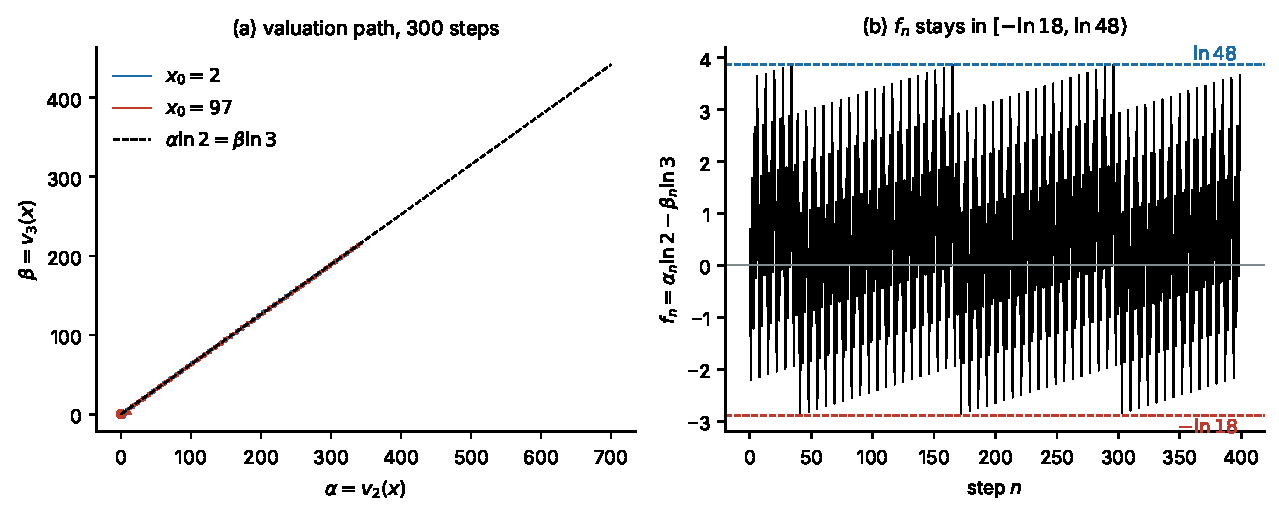
\includegraphics[width=.98\textwidth]{../figures/fig2_valuation_plane.pdf}
\caption{(a) The valuation path $(\alpha_n,\beta_n)$ for two starts hugs the line $\alpha\ln2=\beta\ln3$. (b) The quantity $f_n=\alpha_n\ln2-\beta_n\ln3$ for $x_0=2$ stays in the window $[-\ln18,\ln48)$ (Lemma~\ref{lem:window}).}\label{fig:plane}\end{figure}
\begin{figure}[ht]\centering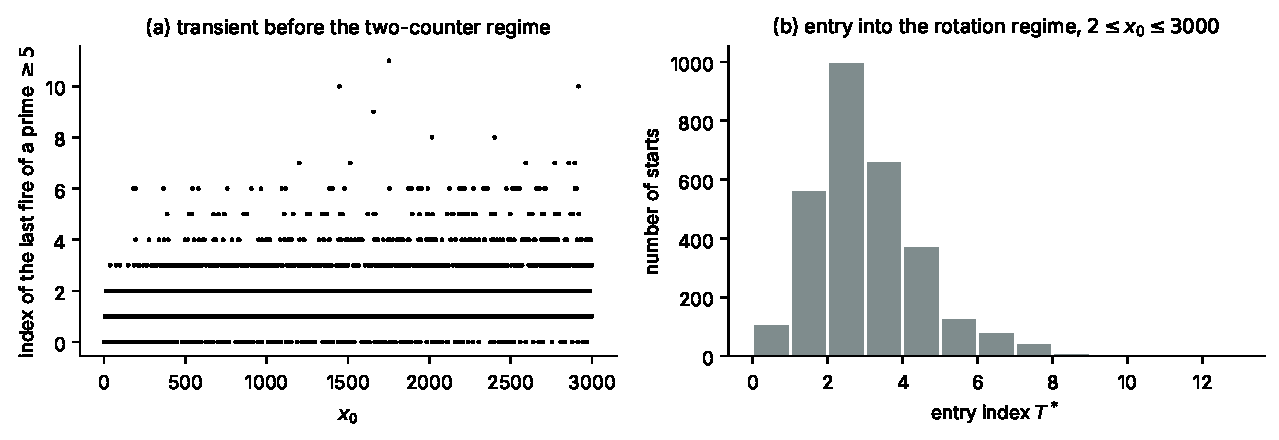
\includegraphics[width=.8\textwidth]{../figures/fig7_transients.pdf}
\caption{(a) Index of the last firing of a prime $\ge5$ for $2\le x_0\le3000$ (computed). (b) Distribution of the entry index $T^*$.}\label{fig:transients}\end{figure}
